\section{Aims and Objectives}
% Load graphicx package in preamble if not already loaded
\graphicspath{{./images/}}

\subsection{Primary Research Question}
This study addresses the following primary research question: \textit{How do urban form, socio-demographic characteristics, and climate factors interact to shape heat vulnerability and health outcomes in Johannesburg, and what interventions could effectively reduce heat-related health impacts?}

Specific sub-questions include: (1) spatial distribution of heat vulnerabilities; (2) mediating factors in heat-health relationships; (3) effectiveness of current adaptation strategies; and (4) optimal infrastructural and policy interventions.

\subsection{Objectives}
This research is structured around three interconnected objectives:

\subsubsection{Objective 1: Geographically Weighted Heat Vulnerability Mapping}
Develop comprehensive spatial vulnerability assessment using geographically weighted approaches that account for spatial non-stationarity. This will identify patterns of heat risk across Johannesburg's diverse urban landscape, examine how historical development patterns shape contemporary vulnerability, and identify priority intervention areas with particular emphasis on infrastructural and socio-spatial inequities.

\subsubsection{Objective 2: Causal Mechanisms of Heat-Health Relationships}
Identify causal mechanisms underlying observed patterns of heat vulnerability through advanced explanatory modeling. This involves investigating which biological systems are most affected by heat stress, how these impacts vary across demographic groups, and what socioeconomic factors mediate these effects.

\subsubsection{Objective 3: Predictive Modeling for Early Warning Systems}
Develop predictive models incorporating near-real-time environmental data, meteorological forecasts, and vulnerability factors to predict heat-health risks. This includes identifying critical temperature thresholds and neighborhood-specific warning indicators to support short-term emergency response and longer-term adaptation planning.

\begin{figure}[h]
    \centering
    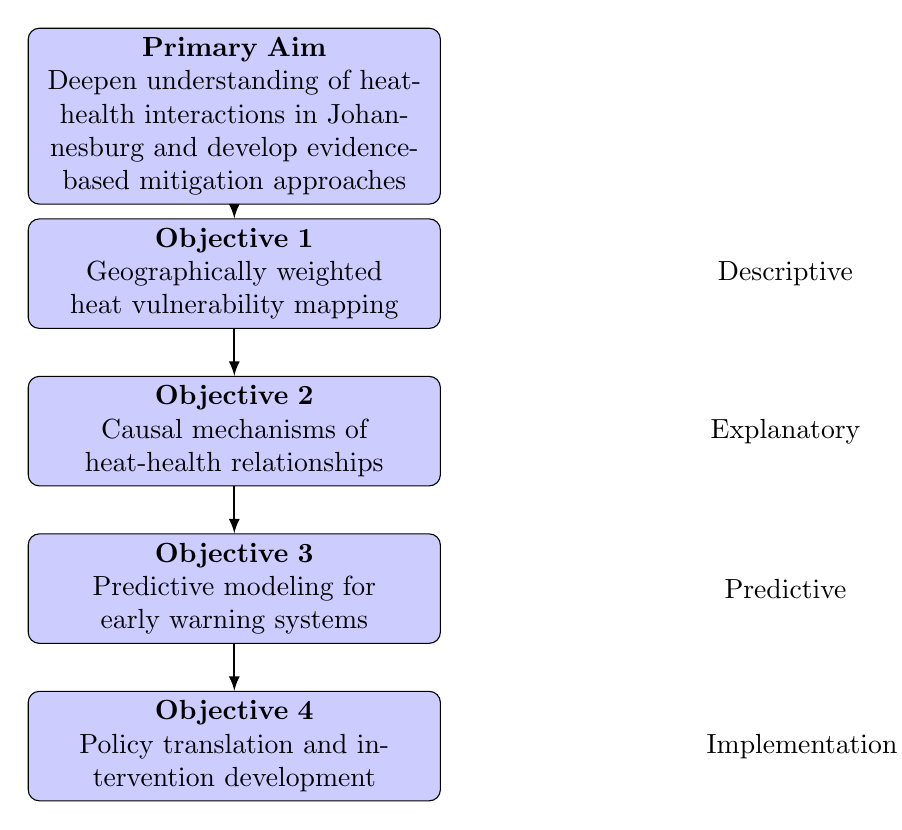
\begin{tikzpicture}[node distance=2cm, auto, 
        block/.style={rectangle, draw, fill=blue!20, text width=5cm, text centered, rounded corners, minimum height=1cm},
        arrow/.style={draw, thick, -latex},
        label/.style={rectangle, draw=none, fill=none, text width=2cm, text centered}
    ]
    % Nodes
    \node[block] (aim) {\textbf{Primary Aim}\\Deepen understanding of heat-health interactions in Johannesburg and develop evidence-based mitigation approaches};
    \node[block, below of=aim, node distance=2cm] (obj1) {\textbf{Objective 1}\\Geographically weighted heat vulnerability mapping};
    \node[block, below of=obj1, node distance=2cm] (obj2) {\textbf{Objective 2}\\Causal mechanisms of heat-health relationships};
    \node[block, below of=obj2, node distance=2cm] (obj3) {\textbf{Objective 3}\\Predictive modeling for early warning systems};
    \node[block, below of=obj3, node distance=2cm] (obj4) {\textbf{Objective 4}\\Policy translation and intervention development};
    
    % Arrows connecting nodes
    \draw[arrow, -latex] (aim) -- (obj1);
    \draw[arrow, -latex] (obj1) -- (obj2);
    \draw[arrow, -latex] (obj2) -- (obj3);
    \draw[arrow, -latex] (obj3) -- (obj4);
    
    % Labels with better positioning and styling
    \node[label] at (7,-2) {Descriptive};
    \node[label] at (7,-4) {Explanatory};
    \node[label] at (7,-6) {Predictive};
    \node[label] at (7,-8) {Implementation};
    
    \end{tikzpicture}
    \caption{Hierarchical framework of research objectives showing progression from descriptive to implementation approaches.}
    \label{fig:framework}
\end{figure}



These four objectives form an integrated research framework addressing spatial, physiological, temporal, and policy dimensions of heat vulnerability. The research design builds each objective upon the findings of the previous one, creating a cohesive pathway from vulnerability characterization to mechanistic understanding to practical solution development.